\section{Auswertung}
\label{sec:Auswertung}

  \subsection{Verdampfungswärme von Wasser bis 1 bar}
  Der zu Anfang gemessene Umgebungsdruck $p_0$ beträgt $985\,\unit{\milli\bar}$. Die gemessenen Werte für das Druckverhalten bei ansteigendender Temperatur für 
  Druck unter 1 bar ist in Tabelle (\ref{tab:Druck_unter_1_bar}) aufgelistet. 

    \begin{table}[H]
      \centering
      \caption{Gemessener Druck $p$ bei verschiedenen Temperaturen $T$}
      \label{tab:Druck_unter_1_bar}
      \begin{tblr}{colspec={c c c c}}
          \toprule
          $T \, \left[\unit{\celsius}\right]$ & $p \, \left[\unit{\milli\bar}\right]$ & $T \, \left[\unit{\celsius}\right]$ & $p \, \left[\unit{\milli\bar}\right]$ & $T \, \left[\unit{\celsius}\right]$ & $p \, \left[\unit{\milli\bar}\right]$\\ 
          \midrule
          25 \pm 1 & 95 \pm 1   & 51 \pm 1 & 197 \pm 1 & 77 \pm 1 & 438 \pm 1 \\                     
          26 \pm 1 & 98 \pm 1   & 52 \pm 1 & 202 \pm 1 & 78 \pm 1 & 453 \pm 1 \\                               
          27 \pm 1 & 102 \pm 1  & 53 \pm 1 & 207 \pm 1 & 79 \pm 1 & 471 \pm 1 \\                   
          28 \pm 1 & 105 \pm 1  & 54 \pm 1 & 212 \pm 1 & 80 \pm 1 & 487 \pm 1 \\                   
          29 \pm 1 & 108 \pm 1  & 55 \pm 1 & 218 \pm 1 & 81 \pm 1 & 507 \pm 1 \\                  
          30 \pm 1 & 112 \pm 1  & 56 \pm 1 & 225 \pm 1 & 82 \pm 1 & 528 \pm 1 \\                   
          31 \pm 1 & 116 \pm 1  & 57 \pm 1 & 231 \pm 1 & 83 \pm 1 & 547 \pm 1 \\                   
          32 \pm 1 & 119 \pm 1  & 58 \pm 1 & 237 \pm 1 & 84 \pm 1 & 578 \pm 1 \\                   
          33 \pm 1 & 122 \pm 1  & 59 \pm 1 & 245 \pm 1 & 85 \pm 1 & 592 \pm 1 \\                   
          34 \pm 1 & 126 \pm 1  & 60 \pm 1 & 252 \pm 1 & 86 \pm 1 & 612 \pm 1 \\                   
          35 \pm 1 & 131 \pm 1  & 61 \pm 1 & 258 \pm 1 & 87 \pm 1 & 635 \pm 1 \\                   
          36 \pm 1 & 134 \pm 1  & 62 \pm 1 & 265 \pm 1 & 88 \pm 1 & 656 \pm 1 \\                   
          37 \pm 1 & 138 \pm 1  & 63 \pm 1 & 273 \pm 1 & 89 \pm 1 & 678 \pm 1 \\                   
          38 \pm 1 & 141 \pm 1  & 64 \pm 1 & 281 \pm 1 & 90 \pm 1 & 700 \pm 1 \\                   
          39 \pm 1 & 145 \pm 1  & 65 \pm 1 & 290 \pm 1 & 91 \pm 1 & 724 \pm 1 \\                   
          40 \pm 1 & 149 \pm 1  & 66 \pm 1 & 299 \pm 1 & 92 \pm 1 & 753 \pm 1 \\                  
          41 \pm 1 & 153 \pm 1  & 67 \pm 1 & 308 \pm 1 & 93 \pm 1 & 775 \pm 1 \\                   
          42 \pm 1 & 157 \pm 1  & 68 \pm 1 & 317 \pm 1 & 94 \pm 1 & 809 \pm 1 \\                   
          43 \pm 1 & 162 \pm 1  & 69 \pm 1 & 327 \pm 1 & 95 \pm 1 & 835 \pm 1 \\                   
          44 \pm 1 & 166 \pm 1  & 70 \pm 1 & 337 \pm 1 & 96 \pm 1 & 867 \pm 1 \\                   
          45 \pm 1 & 170 \pm 1  & 71 \pm 1 & 348 \pm 1 & 97 \pm 1 & 899 \pm 1 \\                    
          46 \pm 1 & 174 \pm 1  & 72 \pm 1 & 360 \pm 1 & 98 \pm 1 & 938 \pm 1 \\                   
          47 \pm 1 & 178 \pm 1  & 73 \pm 1 & 373 \pm 1 & 99 \pm 1 & 989 \pm 1 \\                   
          48 \pm 1 & 183 \pm 1  & 74 \pm 1 & 387 \pm 1 & 100 \pm 1 & 999 \pm 1 \\                   
          49 \pm 1 & 187 \pm 1  & 75 \pm 1 & 401 \pm 1 & & \\ 
          50 \pm 1 & 192 \pm 1  & 76 \pm 1 & 417 \pm 1 & & \\ 
                   
          \bottomrule
      \end{tblr}
    \end{table}
    \begin{figure}
      \centering
      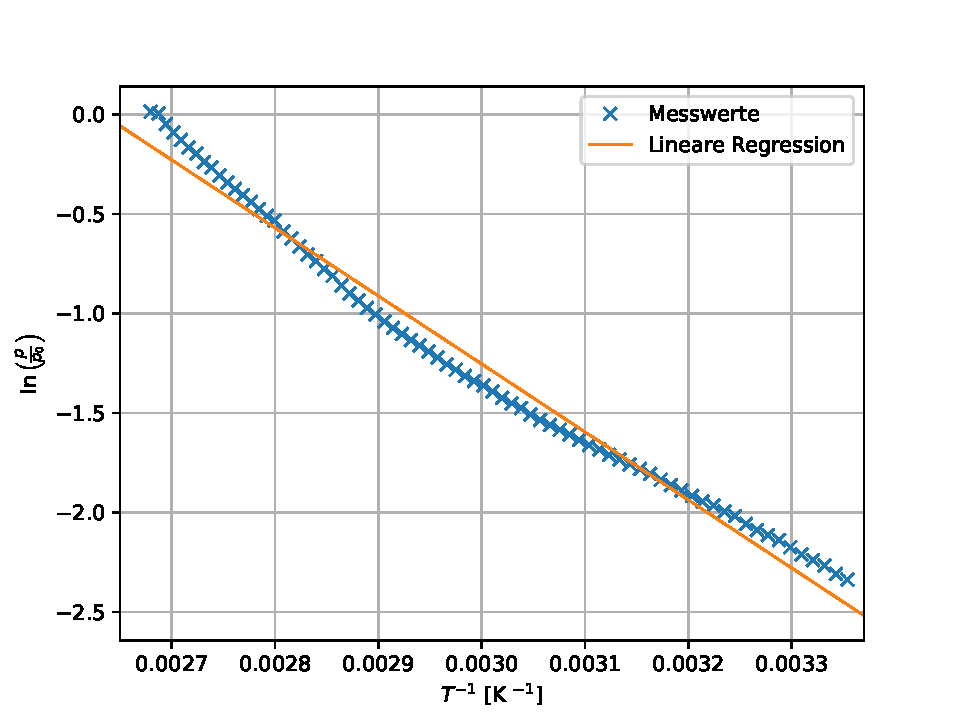
\includegraphics{plot1.pdf}
      \caption{Plot.}
      \label{fig:plot}
    \end{figure}

%Siehe \autoref{fig:plot}!